\newpage
\section{Question 2 - Dataset 1}
\subsection{Introduction}
This report analyzes a dataset containing various features related to restaurants and their revenue. The goal is to explore relationships between different variables and the revenue, and to generate insights that may help in predicting future revenue for restaurants.

\subsection{Dataset Overview}
The dataset contains 8,368 records of restaurants with the following key features:
\begin{itemize}
    \item \textbf{Name}: Name of the restaurant.
    \item \textbf{Location}: The location of the restaurant (Downtown, Rural, Suburban).
    \item \textbf{Cuisine}: The type of cuisine offered by the restaurant (e.g., American, Italian, Japanese).
    \item \textbf{Rating}: Average rating of the restaurant (scale of 1 to 5).
    \item \textbf{Seating Capacity}: The number of seats available at the restaurant.
    \item \textbf{Average Meal Price}: The average price of a meal.
    \item \textbf{Marketing Budget}: The marketing budget of the restaurant.
    \item \textbf{Social Media Followers}: Number of social media followers.
    \item \textbf{Chef Experience}: The number of years of experience the chef has.
    \item \textbf{Number of Reviews}: Total number of reviews received.
    \item \textbf{Average Review Length}: The average length of the reviews.
    \item \textbf{Ambience Score}: Score reflecting the ambience of the restaurant (scale of 1 to 10).
    \item \textbf{Service Quality Score}: Score reflecting the quality of service (scale of 1 to 10).
    \item \textbf{Parking Availability}: Whether parking is available (Yes/No).
    \item \textbf{Weekend Reservations}: Number of reservations during weekends.
    \item \textbf{Weekday Reservations}: Number of reservations during weekdays.
    \item \textbf{Revenue}: The total revenue generated by the restaurant.
\end{itemize}
\subsubsection{Data Cleaning}
The dataset had no missing values, so the main focus was on transforming categorical variables like \textit{Location}, \textit{Cuisine}, and \textit{Parking Availability} into factors for analysis. Imputations for missing values would involve replacing them with median values if necessary.

\subsubsection{Descriptive Statistics}
Table \ref{tab:descriptive} provides a summary of key statistics for the numeric variables in the dataset.

\begin{table}[H]
\centering
\caption{Descriptive Statistics of the Dataset}
\label{tab:descriptive}
\begin{tabular}{lrrrrr}
\toprule
Variable & Mean & Median & Min & Max & SD \\
\midrule
Revenue (in \$) & 656,070 & 604,242 & 184,709 & 1,531,868 & 267,414 \\
Rating & 4.01 & 4.00 & 3.00 & 5.00 & 0.50 \\
SeatingCapacity & 60.21 & 60.00 & 30.00 & 90.00 & 16.57 \\
AverageMealPrice (in \$) & 47.90 & 45.53 & 25.00 & 76.00 & 13.86 \\
MarketingBudget (in \$) & 3,218 & 2,846 & 604 & 9,978 & 1,673 \\
SocialMediaFollowers & 36,191 & 32,519 & 5,277 & 103,777 & 19,830 \\
ChefExperience (Years) & 10.05 & 10.00 & 1 & 19 & 5.47 \\
NumberofReviews & 523 & 528 & 50 & 999 & 275 \\
\bottomrule
\end{tabular}
\end{table}
\newpage
\subsubsection{Data Visualization}
\paragraph{Revenue vs. Average Meal Price}
The relationship between revenue and average meal price is visualized in Figure \ref{fig:revenue_price}. A positive linear trend can be observed, suggesting that restaurants with higher average meal prices tend to generate more revenue.

\begin{figure}[H]
\centering
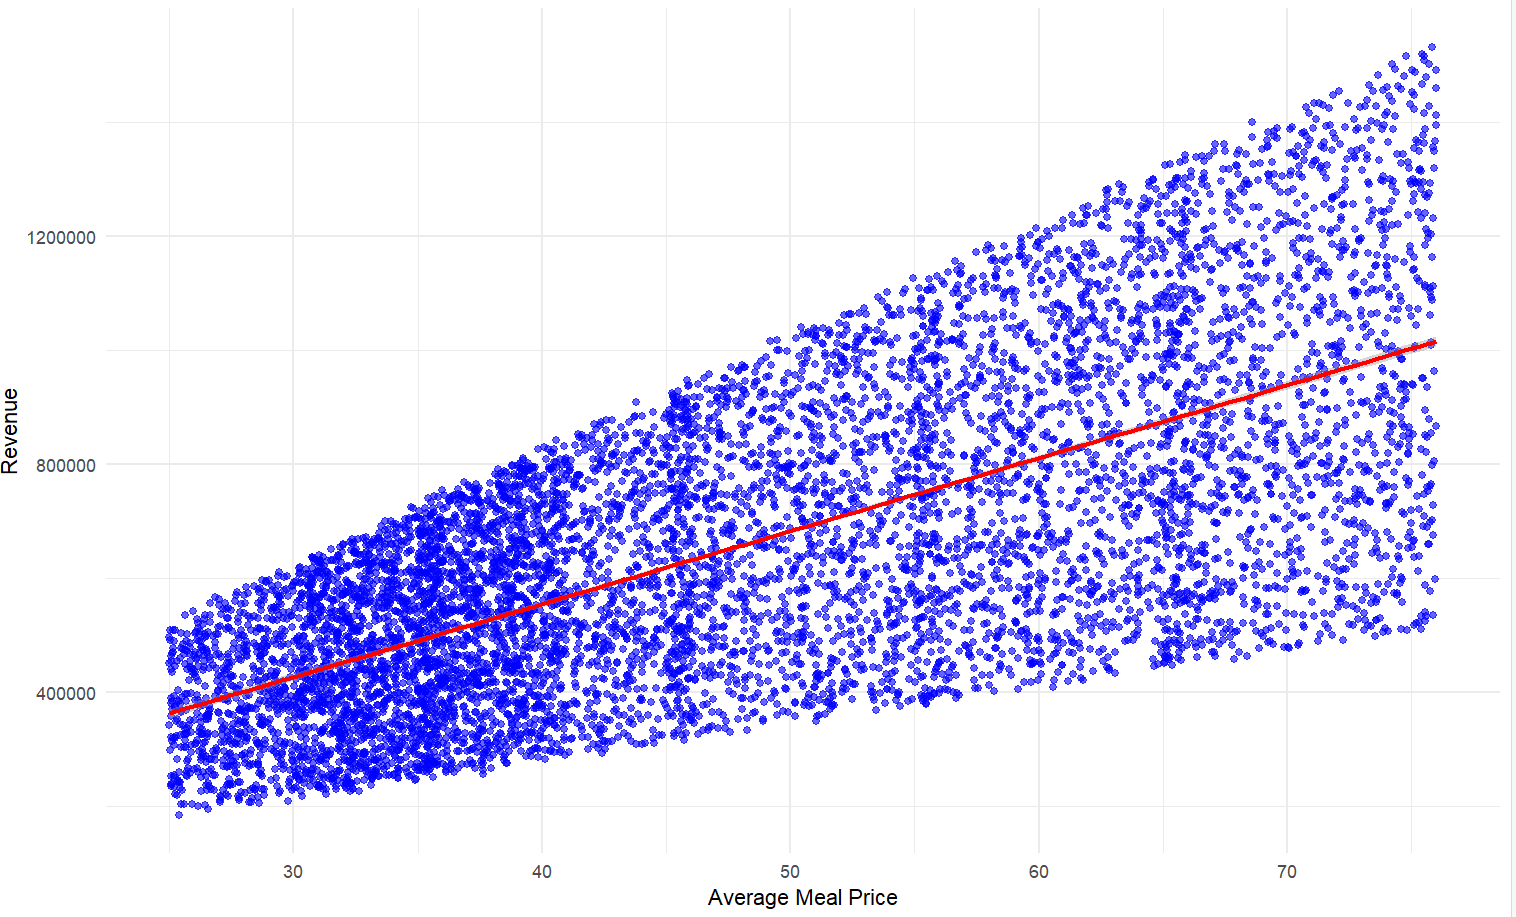
\includegraphics[width=0.7\textwidth]{img/d1.png}
\caption{Scatter Plot: Revenue vs. Average Meal Price}
\label{fig:revenue_price}
\end{figure}

\paragraph{Revenue by Cuisine Type}
Figure \ref{fig:revenue_cuisine} shows the distribution of revenue across different cuisine types. Certain cuisines, such as Japanese and French, tend to have higher median revenues.

\begin{figure}[H]
\centering
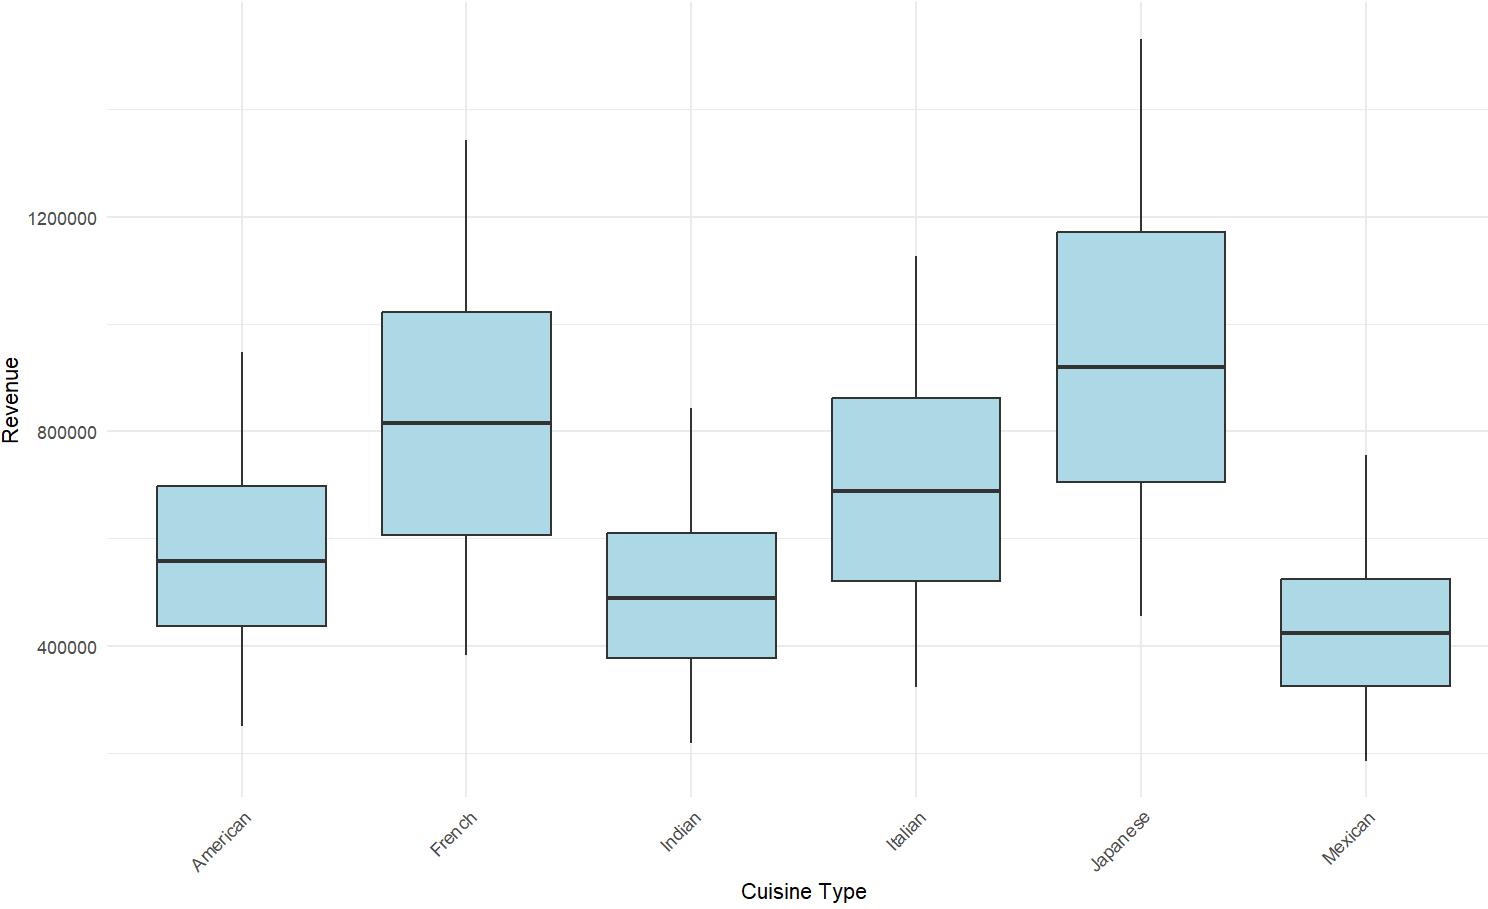
\includegraphics[width=0.7\textwidth]{img/d2.png}
\caption{Boxplot: Revenue by Cuisine Type}
\label{fig:revenue_cuisine}
\end{figure}

\subsubsection{Correlation Analysis}
A correlation analysis was conducted to identify relationships between numeric variables. Figure \ref{fig:correlation} presents a correlation heatmap that highlights strong correlations, such as between seating capacity and revenue, and between average meal price and revenue.

\begin{figure}[H]
\centering
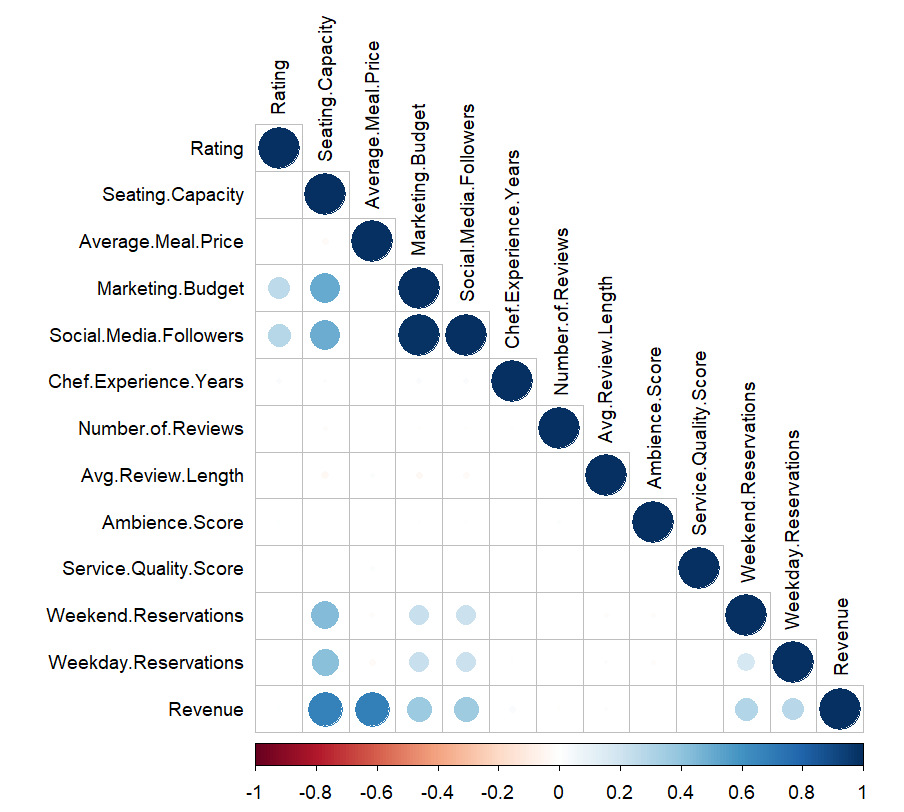
\includegraphics[width=0.7\textwidth]{img/d3.png}
\caption{Correlation Matrix}
\label{fig:correlation}
\end{figure}
\subsubsection{Distribution of Scaled Revenue}
The distribution of scaled revenue (revenue divided by seating capacity) is visualized in Figure \ref{fig:scaled_revenue_distribution}. This metric helps normalize revenue across restaurants of different sizes, providing a more equitable comparison.

\begin{figure}[H]
\centering
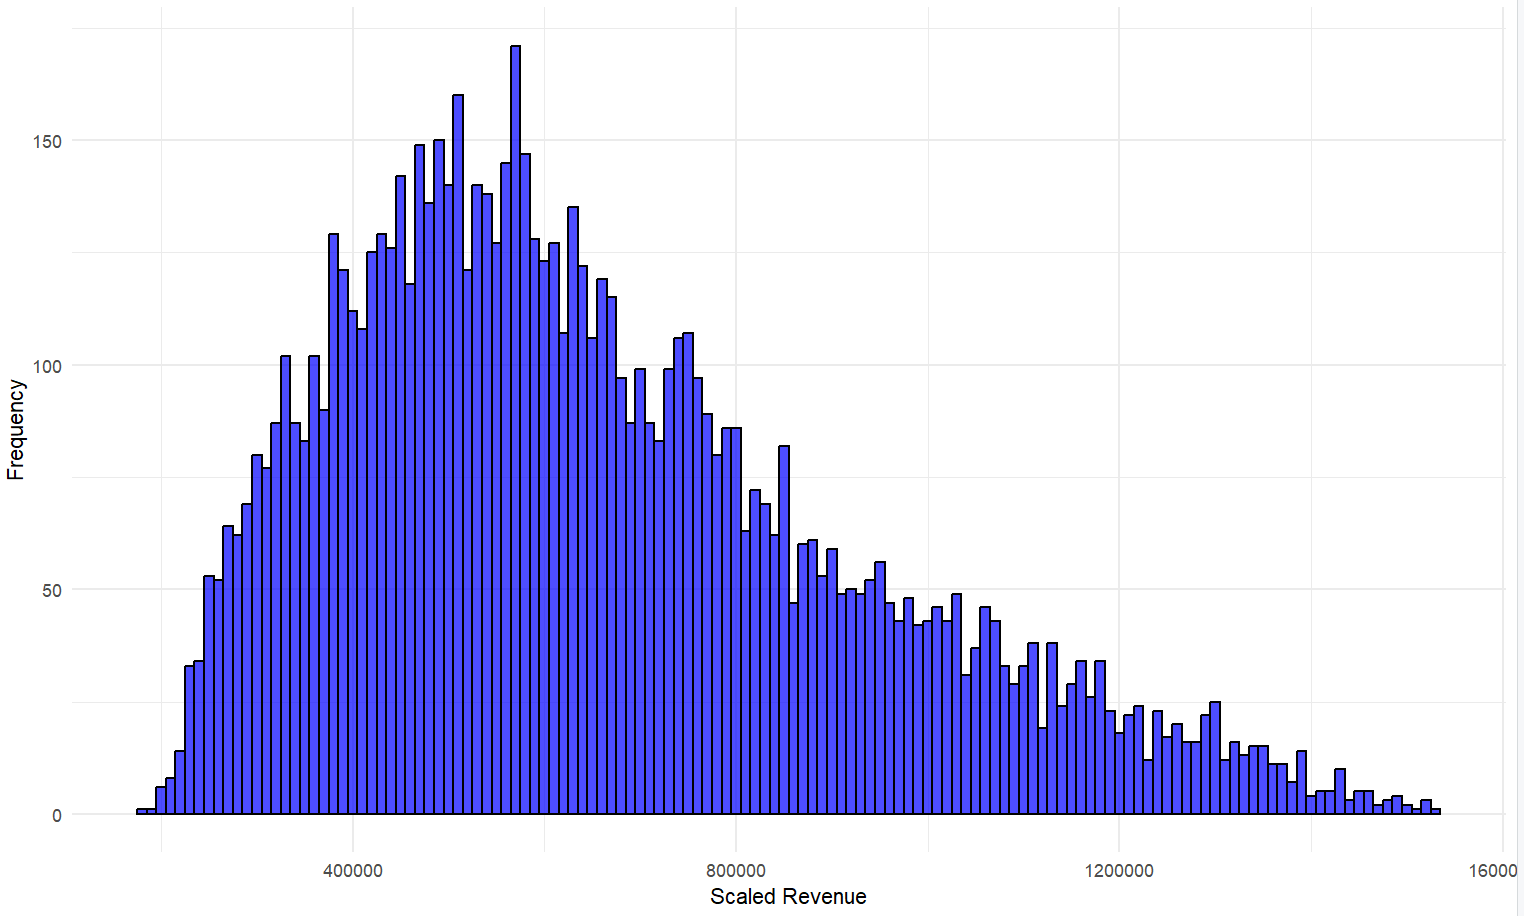
\includegraphics[width=0.7\textwidth]{img/d4.png}
\caption{Histogram: Distribution of Scaled Revenue (Revenue per Seat)}
\label{fig:scaled_revenue_distribution}
\end{figure}

The histogram shows that while most restaurants fall within a certain range of scaled revenue, there are a few outliers with significantly higher or lower revenue per seat. This could be indicative of unique business models or market conditions.

\subsection{Data splitting}

The data is split into two part, training dataset and validation dataset. Training dataset contains 80$\%$ of the observations and the validation dataset contains 80$\%$ of the observations. The split is performed randomly with RStudio.

For replication, we use the seed 777489.

\subsection{Model building}
\subsubsecction{Baseline model}
When inspecting the interaction between indicators, we notice that the interaction term between 'SeatingCapacity' and 'AverageMealPrice' can practically determines 'Revenue' alone, as shown by the plot below:

\begin{figure}[H]
\centering
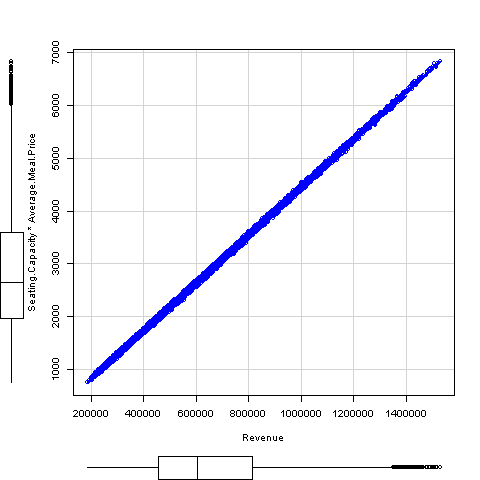
\includegraphics[width=0.7\textwidth]{img/scattertrip.png}
\caption{Scatterplot: Revenue by SeatingCapacity*AverageMealPrice}
\label{fig:scaled_revenue_distribution}
\end{figure}

Thus, we choose the baseline model to be: 
\begin{center}
$
M: \ Revenue \ = \beta_0 + \beta_1 \left(\text{SeatingCapacity} \times(\text{AverageMealPrice})\right)
$
\end{center}

\subsection{Improvement to a new model}

So our baseline model have the form of:

\begin{center}
$
M: \ Revenue \ = \beta_0 + \beta_1 \left(\text{SeatingCapacity} \times(\text{AverageMealPrice})\right)
$
\end{center}

So with such a high $R^2$ and such simple formula for the baseline, it is unneccessary to construct a improved model. In addition, to build a model with $R^2$ and adjust $R^2$ surpassing $99,9\%$ is no simple task. 

Hence, the main aim for our new model is to fix a problem of the baseline model: The error of the baseline model is not normal distributed. As many statistical tests, like t-tests and F-tests, rely on the assumption of normally distributed errors. These tests allow us to draw inferences about population parameters based on sample data. 

Luckily, as our baseline model has high $R^2$ and adjust $R^2$ already, we can sacrifice some accuracy for normalizing the error.

\subsubsection{Addition of indicators}
We start by determine which other variables can indicate the 'Revenue'. From all the indicators available, only 'WeekdayReservation' and 'WeekendReservation' shows signs of indication, but not so much. 
\begin{figure}[H]
\centering
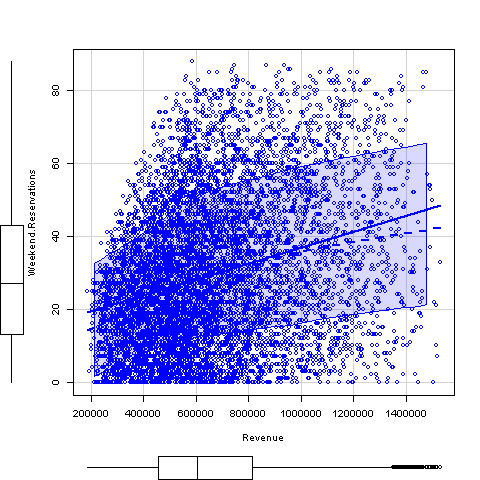
\includegraphics[width=0.7\textwidth]{img/scatterthat.png}
\caption{Scatterplot: Revenue by Reservation}
\label{fig:scaled_revenue_distribution_reservation}
\end{figure}

Drawing the histogram of the two, we also see that while the distribution is fairly normalized, it is skewed. 
\begin{figure}[H]
\centering
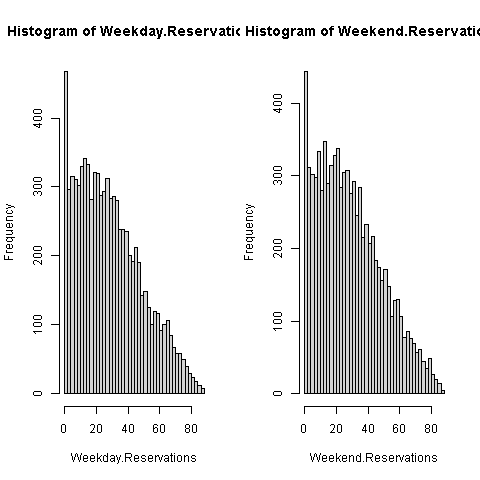
\includegraphics[width=0.7\textwidth]{img/scatterthis.png}
\caption{Histogram of the reservations}
\label{fig:scaled_hist_distribution_reservation}
\end{figure}
Therefore, we perform boxcox transformation on the two of them and indicate the $\lambda$ value to be close to 0.5. As a result, we add the two terms $\sqrt{WeekdayReservation}$ and $\sqrt{WeekdayReservation}$ into the model.

\subsubsection{Interaction terms}
In order to improve the model to ensure the normality of the residuals, we inspect the interaction terms between a quantitative indicator and a qualitative one. After checking all the interaction terms we can, we conclude that the interaction terms that have an impact on the response is SeatingCapacity*Location and AverageMealPrice*Cuisine, as shown by the graphs below:
\begin{figure}[H]
\centering
\begin{subfigure}{.5\textwidth}
  \centering
  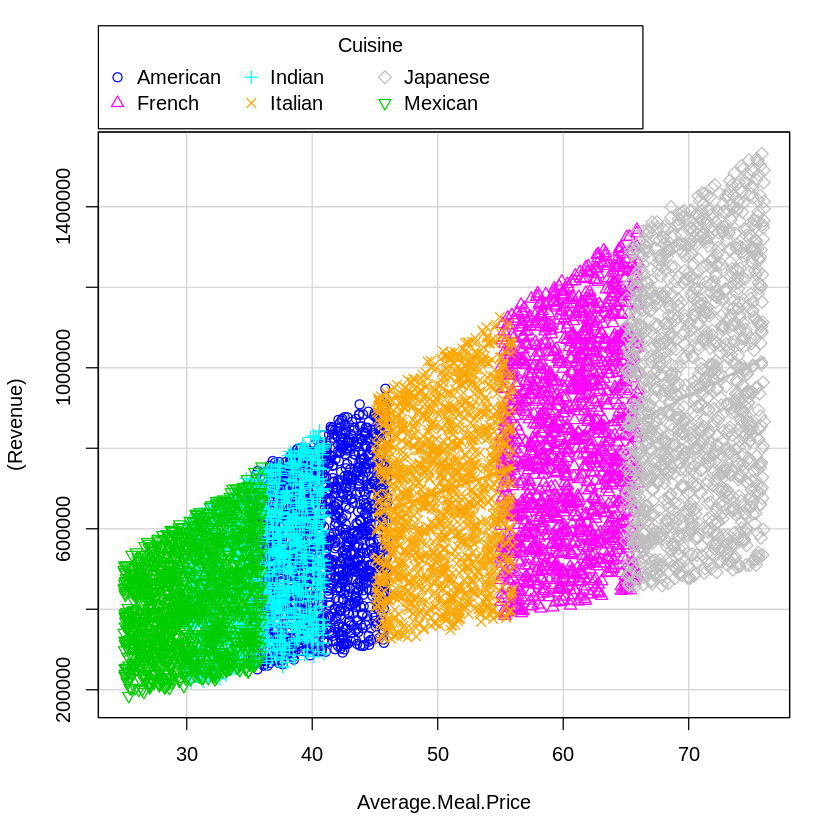
\includegraphics[width=.4\linewidth]{img/revByMealGroupCuisine.png}
\end{subfigure}%
\begin{subfigure}{.5\textwidth}
  \centering
  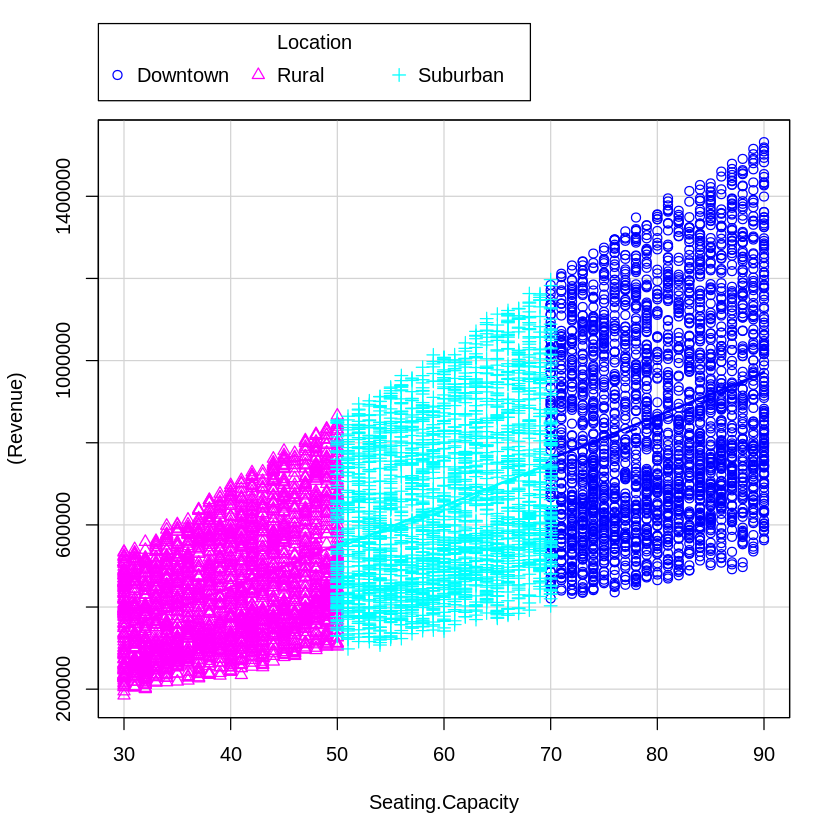
\includegraphics[width=.4\linewidth]{img/revBySeatGroupLocation.png}
\end{subfigure}
\caption{Scatterplot: Revenue by SeatingCapacity grouped by Location and AverageMealPrice grouped by Cuisine}
\label{fig:scaled_revenue_distribution_seatingcapacity_location}
\end{figure}
Therefore, we will add this in the model for further checking.

\subsubsection{Transformation of Average Meal Price}

We examine the Box Cox plot of weight:

\begin{figure}[H]
\centering
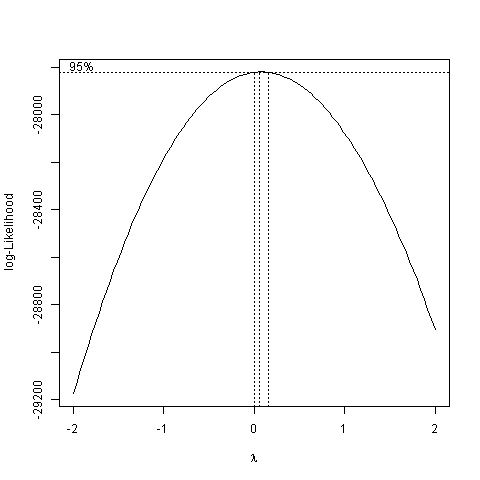
\includegraphics[scale=0.4]{img/Averboxcox.png}
\label{fig:my_label_with_H}
\caption{Box Cox plot of Average Meal Price}
\end{figure}

As Average Meal Price box cox interval is almost 0. We decide to apply the log transformation to it.

\subsubsection{Result model}

From the previous section, we have the new model:
\begin{center}
$
Revenue \ = \beta_0 + \beta_1 \left(\text{SeatingCapacity} \times \log(\text{AverageMealPrice})\right) + \beta_2 \left(\text{SeatingCapacity} \times \text{Location}\right) + \beta_3 \left(\log(\text{AverageMealPrice}) \times \text{Cuisine}\right) + \beta_4 \sqrt{\text{WeekdayReservations}} + \beta_5 \sqrt{\text{WeekendReservations}} + \epsilon
$
\end{center}

Putting this model through stepwise procedure we got the same model.

\begin{table}[ht]
\centering
\captionof{table}{Restaurant model summary}
\begin{tabular}{rrrrr}
  \hline
 & Estimate & Std. Error & t value & Pr($>$$|$t$|$) \\ 
  \hline
(Intercept) & -148660.8591 & 5420.5851 & -27.43 & 0.0000 \\ 
  sqrt(Weekday.Reservations) & -647.7837 & 316.8199 & -2.04 & 0.0409 \\ 
  sqrt(Weekend.Reservations) & -842.6644 & 323.4639 & -2.61 & 0.0092 \\ 
  Seating.Capacity:log(Average.Meal.Price) & 3110.1851 & 18.1174 & 171.67 & 0.0000 \\ 
  Seating.Capacity:LocationRural & 984.2925 & 69.6286 & 14.14 & 0.0000 \\ 
  Seating.Capacity:LocationSuburban & 285.8088 & 30.4116 & 9.40 & 0.0000 \\ 
  log(Average.Meal.Price):CuisineFrench & 47357.0901 & 515.9533 & 91.79 & 0.0000 \\ 
  log(Average.Meal.Price):CuisineIndian & -10379.0297 & 587.1932 & -17.68 & 0.0000 \\ 
  log(Average.Meal.Price):CuisineItalian & 24025.5973 & 535.5268 & 44.86 & 0.0000 \\ 
  log(Average.Meal.Price):CuisineJapanese & 69096.7374 & 514.4629 & 134.31 & 0.0000 \\ 
  log(Average.Meal.Price):CuisineMexican & -21938.8074 & 626.6495 & -35.01 & 0.0000 \\ 
   \hline
\end{tabular}
\\
Multiple R-squared:  0.9659 \\
Adjusted R-squared:  0.9659 \\
\end{table}

Hence, we check the error normality assumption of this resulting model and our baseline.

\begin{table}[H]
\centering
\captionof{table}{Shapiro-Wilk test result}
\begin{tabular}{lll}
  \hline
         &       W             & p-value    \\
    \hline
        Baseline & 0.98703 & 4.078e-11
        Improved model & 0.99837 & 0.1033 \\
   \hline
\end{tabular}
\label{tab:vif}
\end{table}

So our new model preserve the error normality assumption.

\subsection{Hypothesis testing}

Before proceeding, we rewrite our model a little bit:

\begin{center}
$
M: \ Revenue \ = \beta_0 + \beta_1 \left(\text{SeatingCapacity} \times \log(\text{AverageMealPrice})\right) + \beta_2 \left(\text{SeatingCapacity} \times \text{Location}\right) + \beta_3 \left(\log(\text{AverageMealPrice}) \times \text{Cuisine}\right) + \beta_4 \sqrt{\text{WeekdayReservations}} + \beta_5 \sqrt{\text{WeekendReservations}} + \epsilon
$
\end{center}

\subsubsection{Model utility}

We are testing the hypothesis:

\begin{center}
    $H_0: \beta_i = 0, i \in \{1,2,3,4,5\}$
    $ \\ $
    $H_1:$ At least one of $\beta_i \neq 0, i \in \{1,2,3,4,5\}$
\end{center}

This mean we are calculating the test statistic value $f= \frac{R^2/k}{1-R^2} \ \frac{1}{(n-(k+1)}$.

Based on the results of your linear regression model, the F-statistic is \( F = 18{,}930 \), which corresponds to a p-value of less than \( 2.2 \times 10^{-16} \). This extremely low p-value indicates that we can confidently reject the null hypothesis (\( H_0 \)) that all the coefficients are zero. Therefore, we can conclude that the model contains a significant linear relationship between the response variable \texttt{Revenue} and at least one of the predictor variables included in the model.


\subsubsection{Error normality assumption}

We are testing the hypothesis of:

\begin{center}
    \( H_0: \epsilon \) is normally distributed \\
    \( H_1: \epsilon \) is not normally distributed
\end{center}

To test this, we can use the test data. Let \texttt{predict\_revenue} be our result after passing the test observation through the model. Let \texttt{revenue} be the corresponding value of that observation. Then, \( \epsilon = \texttt{predict\_revenue} - \texttt{revenue} \). We will run the Shapiro-Wilk test on this resulting error.

Here is the result of our Shapiro-Wilk test:

\begin{table}[H]
\centering
\captionof{table}{Shapiro-Wilk test result}
\begin{tabular}{ll}
  \hline
                W             & p-value    \\
  \hline
        0.99837   & 0.1033   \\
  \hline
\end{tabular}
\label{tab:shapiro}
\end{table}

This means we have failed to reject the hypothesis that \( \epsilon \) is normally distributed.

\subsubsection{Autocorrelation}

We are testing the hypothesis:

\begin{center}
    \( H_0: \) There is no autocorrelation in the error terms of the linear regression model. \\
    \( H_1: \) There is autocorrelation in the error terms of the linear regression model.
\end{center}

To test this, we can run the Durbin-Watson test, which is available in R. After running the test, we get the result:

\begin{table}[H]
\centering
\captionof{table}{Durbin-Watson test result}
\begin{tabular}{ll}
  \hline
                D-W Statistic & p-value    \\
  \hline
        2.012079           & 0.598   \\
  \hline
\end{tabular}
\label{tab:durbin-watson}
\end{table}

This means we have failed to reject the null hypothesis. This indicates that there is no significant autocorrelation in the error terms of the linear regression model.

\subsection{Validation and testing}

We used the same definition of predict$\_$revenue as the previous section. It's the result of passing the test data through our model.

Here is the histogram of predict$\_$revenue:


\begin{figure}[H]
\centering
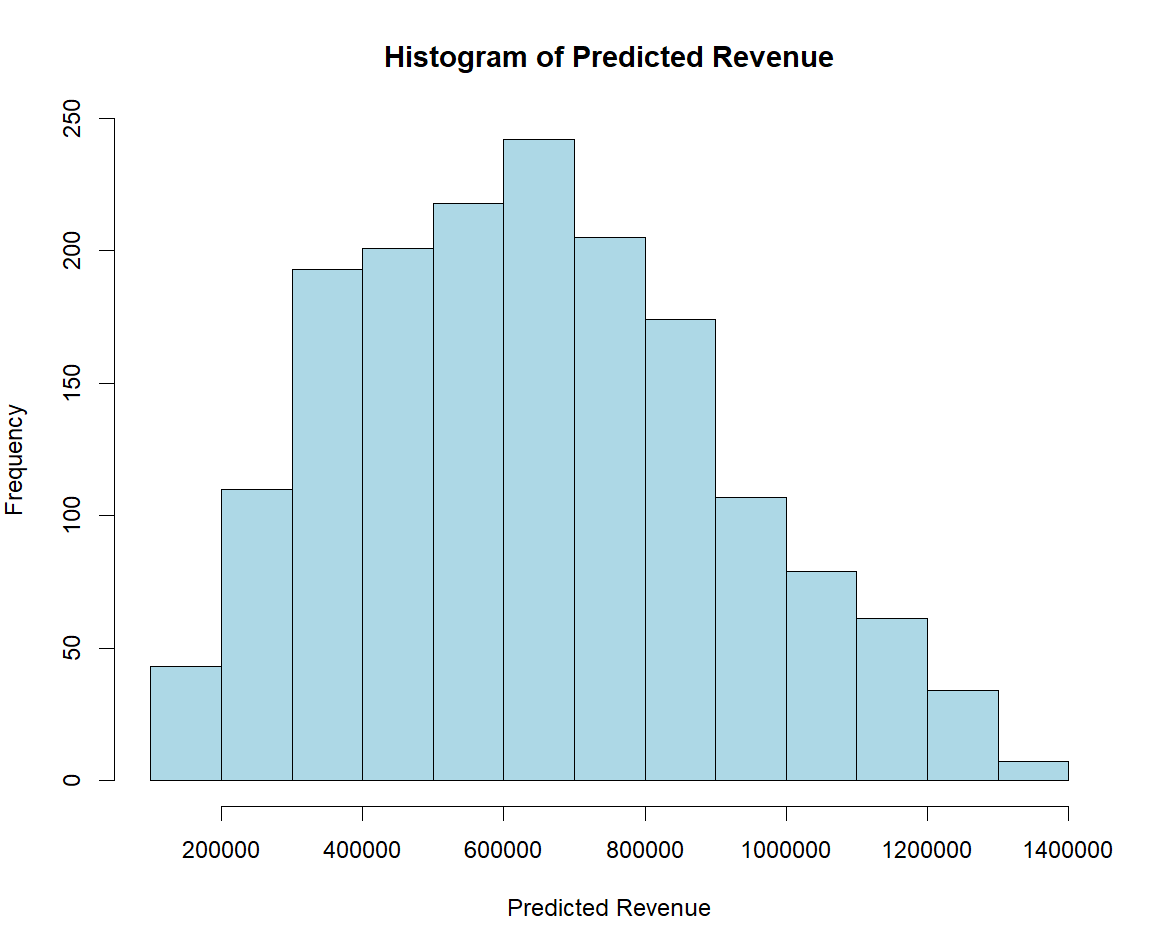
\includegraphics[width=0.7\textwidth]{img/h1b21.png}
\label{fig:scaled_revenue_distribution}
\end{figure}

We compare this to revenue, here is the scatter plot of them:

\begin{figure}[H]
\centering
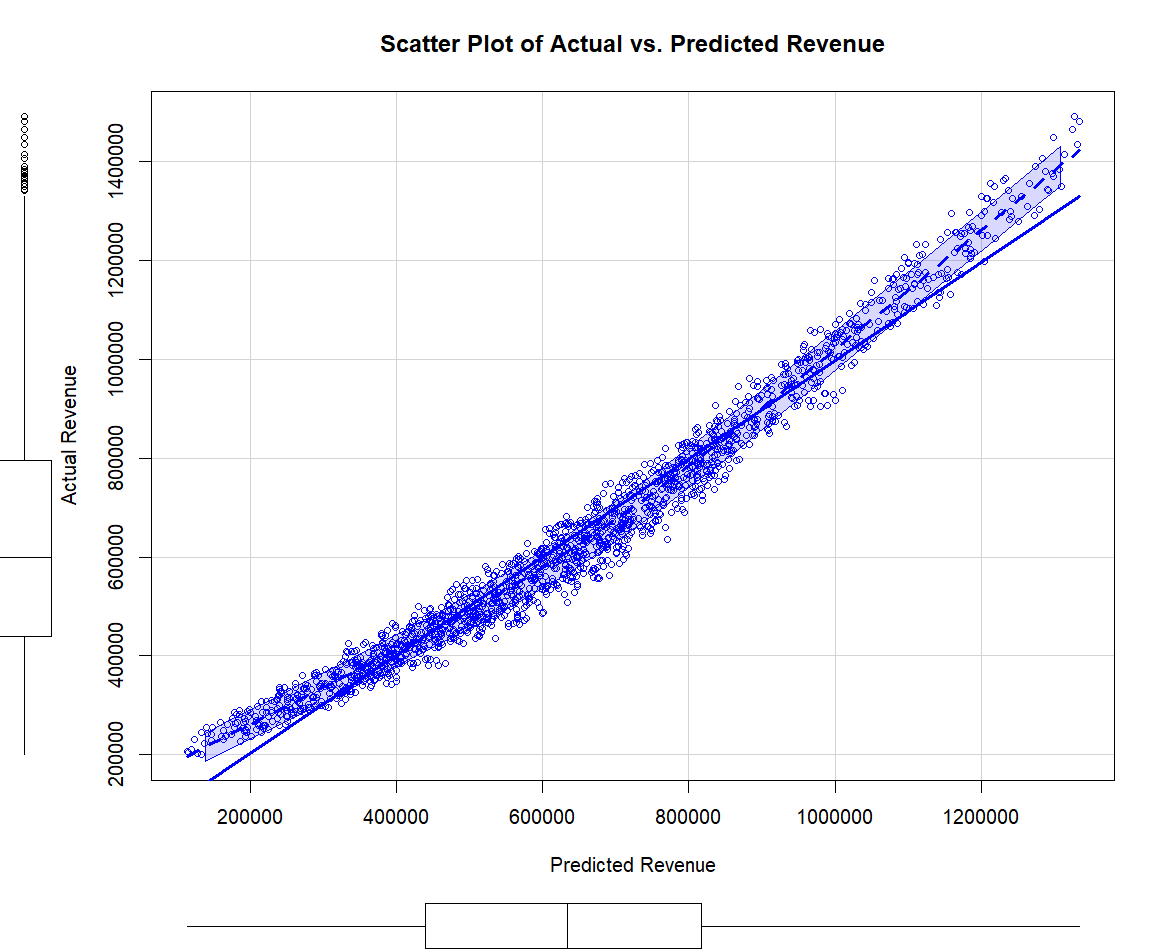
\includegraphics[width=0.7\textwidth]{img/h2b21.png}
\label{fig:scaled_revenue_distribution}
\end{figure}

As they form a almost 45 degree line in the diagonal of the graph, we can say that our model have predict the value of revenue pretty closely.



\subsection{Model Meaning}

Our model is designed to estimate restaurant revenue based on various factors, including seating capacity, meal price, location, cuisine type, and reservation data. The following is our final model:

\begin{center}
$
M: \ \text{Revenue} \ = \ \beta_1 \ + \ \beta_2 \sqrt{\text{Weekday Reservations}} \ + \ \beta_3 \sqrt{\text{Weekend Reservations}} \ + \ \beta_4 \ \text{Seating Capacity} \times \log(\text{Average Meal Price}) \ + \ \beta_5 \ \text{Seating Capacity} \times \text{Location} \ + \ \beta_6 \ \log(\text{Average Meal Price}) \times \text{Cuisine} \ + \ \epsilon
$
\end{center}

With:

\begin{center}
    $\beta_1 = -148660.86$ \\
    $\beta_2 = -647.78$ \\
    $\beta_3 = -842.66$ \\
    $\beta_4 = 3110.19$ \\
    $\beta_5 = \text{Varies by Location}$ \\
    $\beta_6 = \text{Varies by Cuisine}$
\end{center}

Variable Definitions:

\begin{itemize}
    \item Revenue: The restaurant's total revenue.
    \item Weekday Reservations: Number of reservations made during weekdays.
    \item Weekend Reservations: Number of reservations made during weekends.
    \item Seating Capacity: The number of seats available in the restaurant.
    \item Average Meal Price: The average price of a meal at the restaurant.
    \item Location: The location of the restaurant (Urban, Suburban, or Rural).
    \item Cuisine: The type of cuisine served by the restaurant (e.g., French, Indian, Italian, etc.).
\end{itemize}

Key Takeaways:

\begin{itemize}
    \item The initial revenue intercept is -148660.86.
    \item An increase in weekday or weekend reservations tends to decrease revenue slightly.
    \item Larger seating capacity combined with higher meal prices significantly increases revenue.
    \item Location impacts revenue, with rural locations having a higher effect than suburban ones.
    \item The type of cuisine influences the impact of meal price on revenue, with Japanese cuisine showing the highest positive effect.
\end{itemize}

In layman's terms:

\begin{itemize}
    \item Restaurants with more seats and higher-priced meals tend to earn more revenue.
    \item Weekday and weekend reservations slightly reduce revenue, possibly due to operational costs.
    \item Rural restaurants generally have higher revenue compared to suburban ones, when all other factors are the same.
    \item Japanese cuisine is the most lucrative when combined with higher meal prices.
\end{itemize}

Please note that these conclusions are drawn from the dataset used and may not fully represent real-world dynamics. However, within the scope of our data, the model provides accurate estimates of restaurant revenue.
